\subsection{HDR ML Anomaly Challenge - Gravitational Waves}
{{\footnotesize
\noindent A benchmark for detecting anomalous transient gravitational-wave signals, including "unknown-unknowns," using preprocessed LIGO time-series at 4096 Hz. Competitors submit inference models on Codabench for continuous 50 ms segments from dual interferometers. 


\begin{description}[labelwidth=4cm, labelsep=1em, leftmargin=4cm, itemsep=0.1em, parsep=0em]
  \item[date:] 2025-03-03
  \item[version:] v1.0
  \item[last\_updated:] 2025-03
  \item[expired:] unknown
  \item[valid:] yes
  \item[valid\_date:] 2025-03-03
  \item[url:] \href{https://www.codabench.org/competitions/2626/}{https://www.codabench.org/competitions/2626/}
  \item[doi:] 10.48550/arXiv.2503.02112
  \item[domain:]
    - High Energy Physics
  \item[focus:] Detecting anomalous gravitational-wave signals from LIGO/Virgo datasets
  \item[keywords:]
    - anomaly detection
    - gravitational waves
    - astrophysics
    - time-series
  \item[licensing:] NA
  \item[task\_types:]
    - Anomaly Detection
  \item[ai\_capability\_measured:]
    - Novel event detection in physical signals
  \item[metrics:]
    - ROC-AUC
    - Precision/Recall
  \item[models:]
    - Deep latent CNNs
    - Autoencoders
  \item[ml\_motif:]
    - Anomaly Detection
  \item[type:] Dataset
  \item[ml\_task:]
    - Anomaly Detection
  \item[solutions:] Solution details are described in the referenced paper or repository.
  \item[notes:] NSF HDR A3D3 sponsored; prize pool and starter kit provided on Codabench.

  \item[contact.name:] HDR A3D3 Team
  \item[contact.email:] unknown
  \item[results.links.name:] ChatGPT LLM
  \item[fair.reproducible:] Yes
  \item[fair.benchmark\_ready:] Yes
  \item[id:] hdr\_ml\_anomaly\_challenge\_-\_gravitational\_waves
  \item[Citations:] \cite{campolongo2025buildingmachinelearningchallenges}
\end{description}

{\bf Ratings:} ~ \\

\begin{tabular}{p{0.15\textwidth} p{0.07\textwidth} p{0.7\textwidth}}
\hline
Rating & Value & Reason \\
\hline
dataset & 5 & Uses preprocessed LIGO/Virgo time series data at 4096 Hz, publicly available and standard in astrophysics.
 \\
documentation & 4 & Documentation includes challenge instructions, starter kit details, and baseline descriptions,
but could benefit from more thorough tutorials and code walkthroughs.
 \\
metrics & 4 & ROC-AUC, precision, and recall metrics are clearly specified and appropriate for anomaly detection.
 \\
reference\_solution & 4 & Baseline deep latent CNNs and autoencoders are provided and reproducible, but not extensively documented.
 \\
software & 4 & Benchmark platform provided on Codabench with starter kits and submission infrastructure.
Code and baseline models are publicly accessible but not extensively maintained beyond the challenge.
 \\
specification & 4 & Well-defined anomaly detection task on gravitational-wave time series with clear input/output
expectations and challenge constraints.
 \\
\hline
\end{tabular}

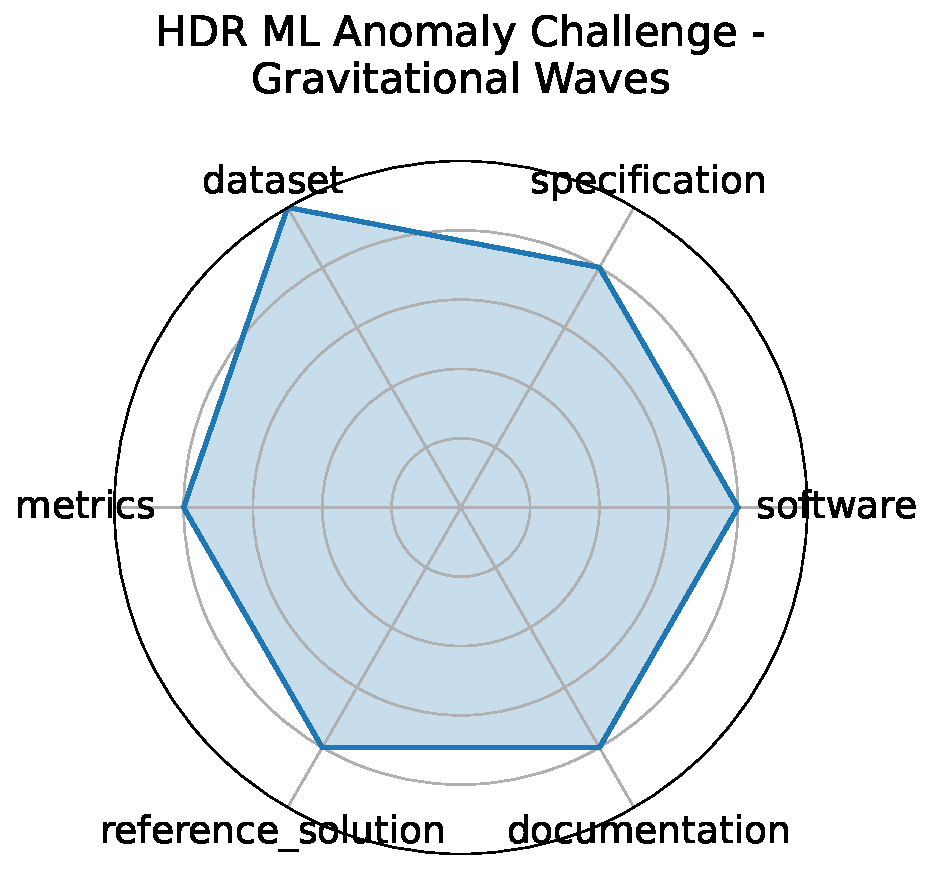
\includegraphics[width=0.2\textwidth]{hdr_ml_anomaly_challenge_-_gravitational_waves_radar.pdf}
}}
\clearpage